\chapter{Magic}

\begin{multicols}{2}

\noindent
A novice miracle worker begins by selecting one of the five paths of magic.
Each path grants access to five spheres -- five collections of spells.

Each level of a sphere typically grants access to a few different spells.
For example, the first level of the Aldaron sphere allows the caster to affect local weather conditions, enchant animals, and summon light.
Divine casters will think of this as a gift from their deity, while blood casters think of these effects as a natural extension of their own will.
However, the basic effects are the same.

\subsubsection{The Spheres of Magic}

\paragraph{Aldaron} allows one to enchant animals then later to harness control of the local weather conditions.

\paragraph{Conjuration} changes things from one form to another, and eventually can summon items out of the air.

\paragraph{Enchantment} allows casters to calm people or panic people. How to confuse and impress them.

\paragraph{Fate} is divine magic and allows the caster to ask a question of the gods, then later to heal companions' \glsentrylongpl{fp}.

\paragraph{Force} magic is a very versatile sphere, allowing the mage to protect themself, fight with levitating weapons or just levitate any object or person.

\paragraph{Illusion} allows the caster to summon apparitions of anything. The caster might hide a door by making an illusion of a wall over it, or create the image of a sleeping bear to frighten people. More skilled illusionists can disguise themselves as other people or creatures.

\paragraph{Invocation} is the magic of fire, lightning and destruction. It begins with bolts of lightning and later allows the caster to incinerate large swathes of enemies with great balls of fire.

\paragraph{Metamagic} is a sphere which enhances all other magical spheres, allowing spells to be cast at long range, then enhancing the mage's mana storage and letting their counter other magical spells.

\paragraph{Necromancy} first deals with making the caster close to death so they can feel no pain and interact safely with the risen dead.
Later the necromancer learns to summon simple spirits into the bodies of the dead to make them rise as an army.

\paragraph{Polymorph} allows the caster to transform into other races, and then into entirely different species.
Exactly which type of animal a caster can transform into depends upon their body type.
Lithe characters will find it easier to turn into a bird, while stronger people will find stronger animals, such as bears or warthogs, easier.

\end{multicols}

\section[Spellcasting]{Casting Your First Spell}

\begin{multicols}{2}

\subsection{Casting}

Spells are cast by spending a number of \gls{mp} equal to the spell's level, so 1st level spells always cost 1 \gls{mp} and 3rd level spells always cost 3 \gls{mp}.
The character then spends the mana and makes a roll against some \gls{tn} to cast the spell.

\index{Mana}\subsection{Mana}

Anyone can buy some base \gls{mp} which is then modified by their Intelligence.\footnote{See the section on Experience, page \pageref{xp}, for costs of base \gls{mp}.} For example, someone with Intelligence +1 who buys Base \gls{mp} 2 would have a store of 3 \gls{mp} to cast spells. Those with a Base \gls{mp} of 0 can still have some \gls{mp} if their Intelligence Bonus is positive.

If a caster has no \gls{mp} left, they can still cast spells by paying the cost with \gls{hp} instead of \gls{mp}.
The magical energies pull the power they need from the blood and bones of the caster, leaving them with a bleeding nose, raging headache and sometimes stranger effects such as acidic pustules or discoloured skin patches.
Many a desperate caster has died through the use of their own magic rather than an enemy's sword; a wizard with their back to the wall is a dangerous opponent indeed.\iftoggle{verbose}{\footnote{\Glsentrylongpl{hp} cannot be spent instead.}}{}

Mana is a fickle thing -- when lazing \ around a village it can take hours to regain even a little driblet of magic.
When fighting in deep caves, a few minutes' focus can summon most of a mage's magical energies back.
Every scene, characters regenerate 2 Mana plus their Wits Bonus.
If this total would be 0 then the amount of time required to gather a single \gls{mp} increases by 1 scene.
Characters with a Wits score of -2 must wait 2 scenes before regenerating 1 \gls{mp} while those with Wits -3 must wait 3 scenes.

\subsection{Range}

\begin{wrapfigure}{r}{.18\textwidth}

\begin{rollchart}

	Wits & Range \\\hline

	-4 & 1 \\

	-3 & 2 \\

	-2 & 3 \\

	-1 & 4 \\

	0 & 5 \\

	1 & 10 \\

	2 & 15 \\

	3 & 20 \\

	4 & 25 \\

\end{rollchart}

\end{wrapfigure}

Spells have a range of 5 squares plus 5 times the caster's Wits bonus.
A negative Wits Bonus decreases the range by one square per penalty.

\iftoggle{verbose}{
Magic extends all around the character but mages can rarely affect targets anywhere near the range of a good archer.
Metamagic can dramatically extend the range, but the basic spell range is always rather close.
}{}

Spells which affect a large area are only restricted by where they \emph{start}.
A \textit{Wide Fireball} covering 3 squares might be cast 5 squares away, but it could extend past that, reaching a total of 7 squares.

This range limitation applies to all magic, including Song magic.
While a tune may carry over the hilltops, the force of the magic usually remains close to the caster.

\subsection{Duration}

Some spells are instant -- a ball of fire flashes from the mage and incinerates someone, or a touch grants the favour of the gods, healing FP -- but most are continuous. Continuous spells can be cancelled at will or maintained indefinitely. However, while they are being maintained, the \gls{mp} required to cast them remains spent, lowering the mage's maximum \gls{mp}.

For example, Tauron the elven sorcerer casts a spell on himself to appear as a gnome -- all the better to blend into surrounding society. He spends 1 \gls{mp}. Later, he enchants an animal to be his companion for 2 \gls{mp}. Normally, his maximum \gls{mp} is 6, but he is currently reduced to a maximum of 3 \gls{mp} so long as he continues to be a bear-riding gnome.

These still-active spells are known as \glspl{standingspell}. Some mages operate by continuously casting different spells and then going `empty' when the mana is gone. Others typically operate with \gls{standingspell} alone, casting everything they might need before the day begins and leaving their useful spells `running' but leaving themselves unable to cast more.

\subsection{Spell Types}

Your standard spell takes a while to cast -- normally 1 \gls{round} per level, so a Level 3 spell would normally take 3 \glspl{round} to complete.  Casters can go slower or faster and gain bonuses or penalties to their roll.

\subsubsection{Ritual Spells}

Mages who take their time over spells can attempt a Ritual Spell -- they cast it as a \gls{restingaction}.\footnote{See page \pageref{restingactions}}.
The mage can gain mana slowly, spending some, drawing more from a mana stone or item, then spending more before finally casting the spell.
The mage can gather a number of \gls{mp} equal to double their normal maximum \gls{mp}, ignoring \glspl{standingspell}.
Ritual spells can also be cast as a team effort -- any number of spell casters who are on the same \gls{path} of magic can cast any spell they all know together.
They can each invest \gls{mp} to create \gls{standingspell}, and thereafter any one of them can cancel the spell.

\subsubsection{Subtle Spells}

Casting an illusion or enchantment on someone with a flashing, loud and generally obvious spell can be quite a give away. Any caster can attempt to cast a spell while simply whispering and moving their hands slowly and subtly.  The \gls{tn} is raised by +2 as this is a very difficult way to cast anything.

People around the mage can still sometimes spot a spell being cast. They use their Wits + Academics in a resisted roll against the mage's Dexterity + Deceit.

\subsubsection{Quick Spells}

Quick spells can be completed fast enough to cast in combat, costing 3 Initiative points plus the level of the spell.
Such spells always force a little `flash and bang' out as the raw magic hits the air.
Some mages create sparks as they cast spells, others summon dark mists -- it all depends upon the Path of Magic the mage is walking.

Quick Spells are challenging, and require the mage know a spell intimately.  They cannot be cast with the mage's highest spell level.  A mage with Polymorph at level 3 cannot cast level 3 as a Quick Spell.

\subsection{Spell Enhancements}

Spells can be changed at a cost.
Each enhancement requires the spell to be cast at a higher level, sometimes many levels higher.
These enhancements always take the form of adjectives.
For example, the first level \textit{Fireball} spell, has the enhancement ``(1) Raging'', meaning the mage can cast a \textit{Raging Fireball}, which would count as a second level spell.

Some spells have their own enhancements, and all of them have two in common.

\enhancement{1}{Wide}
\index{Spell Enhancements!Wide}
The spell extends to cover a wide area -- a total area equal to the spell's level, plus the caster's Wits Bonus.
The squares are always continuous, so a spell targeting four squares could form a $2\times 2$ area, or four continuous squares.

If the spell targets people, one person per square is always a reasonable baseline.

\enhancement{2}{Massive}

The spell spreads across a massive space -- indoors this could be multiple rooms, outdoors it could be a field, or a massive segment of a forest.
Massive spells target a number of areas equal to the spell's level plus the caster's Wits.

\vspace{.3in} 

\noindent Now that the basics are covered, let's have a look at the \glspl{sphere}. There are ten in total, each of which covers a very different range of spells. Most \glspl{sphere} allow the mage to cast a different spell at each level, though some grant multiple spells at each level.

\end{multicols}

\sphere{Aldaron}\index{Magic!Aldaron}

\begin{multicols}{2}

\noindent
The elves are intimately familiar with this sphere, and usually refer to it as a simple skill, like painting or any other trade. They call it simply `the knowledge of trees', though it deals with much more than wood -- animals can be turned into friends and companions, the weather can be controlled and at the ultimate level the forest itself can be called to uproot and give aid to the mage.

\spelllevel

\spell{Forest Song}{Continuous}{Beast Ken}
\noindent
Novices of Aldaron can befriend any beast, make them confused, send them to sleep or send them into a blind panic.
Passive mammals such as sheep are easy to target while aggressive or strange creatures can be very difficult to get to grips with.

The \gls{tn} for this spell is 7 plus the target beast's Wits + Aggression Skill (the Skill which replaces Combat for beasts). The caster rolls their Intelligence + Beast Ken. For example, a creature with Wits +1 and Aggression +2 would be at \gls{tn} 10 to affect.

Mages can use this magic to make animals easier to train, although most animals are not particularly useful -- they cannot tell the mage important information or understand simple commands.

Forest Song works on all creatures without an Intelligence score.
Umber hulks, bears, birds, et c. -- all can be affected with the language of the forest.
However, mammals are the easiest to work with.
The \gls{gm} should add to the \gls{tn} to affect birds, insects and other non-mammalian creatures.

Forest Song replicates the first three levels of the Enchantment Sphere but the targets are beasts rather than people, and the \gls{tn} and Skill is determined by this level, not the enchantment spell.

\enhancement{1}{Binding}

With an additional level added, the spell can replicate all five levels of the Enchantment sphere, but retains the exception that the only Skill used is Beast Ken.
The animals targeted by this spell gain a little rudimentary intelligence -- just enough to carry out commands and relay information.
They still lack any Intelligence bonus.

\spell{Light}{Continuous}{Survival}\\
\label{light}

\iftoggle{verbose}{

	\noindent\includegraphics[width=\linewidth]{images/Roch_Hercka/flashing_light.jpg}
	\label{roch:light}
}{}

The mage casts a dim light, about the strength of a torch, which floats around a single point (but never very steadily).
This light can blind an opponents in the darkness by casting it directly in their face.
Anyone having the werelight flare up in their face becomes blinded for a number of rounds equal to the spell's level minus the target's Wits Bonus.
The average human, having a Wits Bonus of -1, would be blinded for 1 round.
The blindness can be automatically avoided by anyone who was Keeping Edgy (see page \pageref{edgy}), as quickly shielding one's eyes averts any damage.

Undead are terrified of this light.
Those affected by the spell make a Wits + Aggression roll, \gls{tn} 7 plus the caster's Intelligence + Survival.

\spell{Plantform}{Continuous}{Survival}\\
Young plants have a natural destinty.
With this spell, a plant's destined form can be changed.
The caster needs to hold the spell until the plant has fully formed, which can stunt the caster's mana for a year or more.
The affected plant cannot be larger than a man, unless enhancements increase the area of effect.

The caster has various options for how the spell grows the plants:

\paragraph{Edible} plants produce a number of meals equal to the spell's level plus the caster's Intelligence Bonus.
\textit{Wide} spells produce the same amount of food times the spell's level, plus the caster's Wits Bonus.

\paragraph{Poisonous} plants taste the same as the edible plants, but inflict a number of Fatigue Points when ingested equal to the spell's level plus the caster's Wits times 2.\footnote{$(L + Wts)\times 2$}

\paragraph{Wildform} plants are just plants with any shape the caster desires.
They might grow into the form of a chair, or even a house if the spell is large enough.
Anything is plausible if a plant could be carved into the right space.

\spell{Freezing Touch}{Continuous}{Survival}\\
The mage can freeze solid any body of water, or even damage people by cooling their body.

If cast on a person, they take \arabic{spelllevel} Fatigue Points plus the caster's Intelligence Bonus.\footnote{The elvish natural immunity to cold does nothing to prevent this damage.}
Exactly how effective this is depends a lot on how tired the target already is.

Bodies of water freeze over the moment the spell is finished.
Such ice has an effective Strength Bonus of \arabic{spelllevel} plus the caster's Intelligence Bonus, and covers up to \arabic{spelllevel} squares plus the caster's Wits Bonus.
The spell's Strength Bonus can test if the ice can trap people who are in the water, or if it can support people's weight (it holds a maximum \gls{weightrating} of its own Strength +4).

Creatures only frozen up to their waist or ankles can gain a bonus to break out of the ice, and a further bonus if the spell is cast slowly.
If the caster can extend the range, then the spell can travel any distance, although longer distances can make the spell rather a long-shot, with each area traversed raising the \gls{tn} by 3.

\spell{Wind Blast}{Instant}{Survival}\\
Wind can also be made to blow forward in a blast in front of the mage.
The blast spans out, affecting \arabic{spelllevel} squares plus the mage's Wits Bonus.
Each person affected instantly loses 2 Initiative points plus the caster's Intelligence Bonus, minus the targets' Strength Bonus (minimum 1).
The wind can emanate from any location in range and stop at any location in range but any wind coming from behind people will not be effective in slowing them down.
Those affected by such a wind cannot move until their Initiative comes up again, i.e. movement is no longer a Quick Action.
Finally, the wind moves the target back 2 squares plus the caster's Intelligence Bonus minus their Strength Bonus, since larger, heavier creatures are more difficult to move, while smaller creatures (with a negative Strength) move farther.

For example, Darren the druid blasts out a scathing wind against a row of goblins -- his Wits of +2 means he affects \setcounter{list}{2}\addtocounter{list}{\value{spelllevel}}\arabic{list} squares; since his Intelligence is +1, each target would lose each \setcounter{enc}{1}\addtocounter{enc}{\value{spelllevel}}\arabic{enc} points of Initiative, however the goblins' Strength Bonus is -1, so they finally lose \addtocounter{enc}{1}\arabic{enc} points and cannot move until their next Initiative action.
Each moves back (in the direction of the wind) \arabic{enc} squares minus their Strength Bonus -- again, since this is -1 they move back \arabic{enc} squares.

\spelllevel

The mage begins to commune with the weather systems and influence how they go. They can even summon localised weather systems from the palm of a hand; mist, sunlight, wind and more are all possible.

\spell{Air Bubble}{Continuous}{Survival}\\
Weather-workers can summon an air bubble anywhere within range, with a diameter equal to \arabic{spelllevel} squares plus the caster's Wits Bonus. The air bubble can be used to walk underwater without getting wet (though drips through the bubble are common). It will remain despite any damage to its outer `wall' -- penetrating objects simply slip in and out seamlessly. All air bubbles must be summoned while on the land, taking it down below -- any bubbles which begin underwater will simply summon a bubble of stagnant water and will collapse under their own weight once brought onto the land. Air bubbles can also help stop invading winds, mists and such, but with such a limited range their usefulness is also limited.

Any projectiles targeted at the airbubble lose a lot of their power -- arrows, and fireballs both become a little impotent when faced with it.
It provides a total \gls{dr} of \arabic{spelllevel} + Intelligence against all ranged attacks.

\spelllevel

\spell{Forest's Call}{Continuous}{Beast Ken}\\
The caster makes a call to the forest to come and attack the nearby target.  If the target is a player, the \gls{gm} rolls \arabic{spelllevel} times plus the caster's Intelligence on the local encounter table, and the \gls{pc} faces all encounters within the next day, and typically within the next scene.  The \gls{gm} is encouraged to combine all encounters into one.

If the target is an \gls{npc}, they lose \arabic{spelllevel} \gls{fp} + the caster's Intelligence.
If this leaves the target on 0 \gls{fp}, the target meets with an unfortunate accident next time they enter a natural environment, and dies.

The curse only lasts while it's maintained, and only takes effect in a natural environment where creatures roam -- not in towns or otherworldly environments.

\spell{Telos}{Instant}{Survival}\\
The spell reaches out to any plant, dead or alive, and fast-travels it to its natural conclusion.
Seeds grow into plants and blossom, plants grow tall, and older plants whither and die.

\begin{wrapfigure}{r}{.25\textwidth}

	\begin{rollchart}

		Margin & Aging \\\hline
	
		0 & 1 Year \\
	
		1 & 5 Years \\
	
		2 & 1 Decade \\
	
		3 & 5 Decades \\
	
		4 & 1 Century \\
	
		5 & 2 Centuries \\

	\end{rollchart}

\end{wrapfigure}

The result depends upon the margin.

Poorly made weapons with wooden parts collapse once aged a decade.
Most will collapse after 5.

Bushes targeted by the spell can grow tall instantly, while trees can take decades, or even a century to grow to full height.

The spell must target a complete `thing', and never a piece of a thing.
A basic spell can target a sword, therefore destroying its handle with age, but could not target a door in a house -- the entire house would have to be targeted, or the spell would not work.
Spells massive enough to target a building might affect the exterior, but would to nothing to the interior unless it could target every room within as each room counts as its own area.

\end{multicols}

\sphere{Conjuration}

\begin{multicols}{2}

\noindent
Conjuration deals with changing matter.
It starts by shifting water into mud, or stone into ice.  Later the caster can change types of matter -- liquids into solid, solid metal into air, anything simple.
Higher levels are less limited, and complex items like a bow and arrow, or cart, can be made in an instant, as matter's shape can be changed.  Casters soon also learn how to change matter's location, teleporting items from one place to another.

Conjuration uses various skills to cast, but most commonly Crafts for summoning or changing items, or Survival for water or other simple substances.

Conjuration divides the world into three essential forms -- solid, liquid and gas.  Gases are easiest to work with, liquids come shortly after, and solid objects are usually the most difficult to work with.

Conjuration spells targeting larger items are always more difficult.  The \gls{tn} for anything besides a gas, such as air, is always increased by the \gls{weightrating}.
In the case of living targets, the \gls{weightrating} is always equal to their \gls{hp}, so targeting someone with 6 \gls{hp} would increase the \gls{tn} by 6.

Any character can decide that a conjuration spell targeting them fails by spending 5 \gls{fp}, if that spell would be fatal.

\spelllevel

The mage can turn any single, cohesive, target into another of the same type.  Mist can turn to air, or air can turn into mist.
Ice can turn into rock, and water can turn into sludge.

Food substances, gold coins with complex engravings, bows, and other crafted items are too complicated for this spell -- it only transforms matter into something simple of the same type.

\spell{Choking Fog}{Continuous}{Survival}\\
The caster changes the nearby air into a caustic mess.  When cast outdoors the mist disipates at the end of the \gls{round}.  When cast in a windy area, the fog disappears instantly.

Anyone Keeping Edgy can hold their breath.  Others gain \arabic{spelllevel} + the cater's Intelligence in Fatigue points each \gls{round}.

The spell affects a number of areas equal to \arabic{spelllevel} + the caster's Wits.

\spell{Purify Air}{Continuous}{Survival}\\
Smoke, fog, or any other substance can be purified.  The spell affects a number of areas equal to \arabic{spelllevel} + the caster's Wits.

\spell{Stonespell}{Continuous}{Crafts}\\
The caster changes any solid target to stone, ice, or any other simple, solid, substance.  The \gls{tn} is 7 plus the target's \gls{weightrating}.\footnote{A living target's \gls{weightrating} is equal to their \glsentrytext{hp}.}
Once the spell is over, the target turns back to normal.

Anyone may spend 5 \gls{fp} in order to stipulate that the spell fails.

Fast moving items, such as a spear used in combat, are additionally difficult to target.  When in use, whatever skills the wielder is using add to the \glsentrylong{tn}.

Metal cannot be targeted by this spell.

\spell{Slime}{Continuous}{Survival}\\
The caster turns any nearby liquid into a slippery slime.  Anyone running across the area makes a Dexterity + Athletics roll, \gls{tn} 7 + the caster's Intelligence.  Some kind of liquid must be in the right place for the spell to work.

Casters acting quickly often carry their own water.  Throwing water requires 8 initiative for using an item, as usual.

\spell{Web}{Continuous}{Survival}\\
The caster turns any liquid into a vicious, sticky substance.
Anyone coming into the liquid gets stuck, and needs to take a full movement action to try to get free.

Casters roll their Intelligence + Survival at a \gls{tn} of 7 + the target's Strength + Athletics. Alternatively, players can avoid being stuck in the web by rolling Strength + Athletics, at \gls{tn} 7 + the caster's Intelligence + Survival.

Anyone can attempt to break free instead of their usual movement action.

Webbing cannot be used instead of rope -- it's too elastic, and tends to snap when stretched.

\enhancement{1}{Artefact}
The caster can now transform targets into detailed forms.  Air can become a complex, and rich scent.  Solid wood can turn into a sword, or rope.  Water can become beer, wine or even acid.

\enhancement{1}{Metallic}
\index{Spell Enhancements!Metallic}
The caster can now target and create basic metals such as copper, bronze, or iron.  Gold and silver cannot be targeted or created, nor can alloys, or weapons adorned with precious metals.

\enhancement{1}{Transient}
\index{Spell Enhancements!Transient}
The conjuration spells can now move from any type of matter to any other.  Webbing, slime, or acid can be created from any substance except metals.

Casters turning air into rocks can rain a heavy load down on an enemy, inflicting $1D6$ Damage, plus their Intelligence, plus the spell level.

Living creatures turned using Stone Spell into a solid substance, and then turned into air or water using Form Breach, are dead.

\spelllevel

Level 2 conjuration can use all the enhancements of the previous level.

\spell{Acid}{Continuous}{Academics}\\
The caster can turn any liquid into a potent acid.
If the acid achieves a Vitals Shot, it gets around armour or clothing, and deals $1D6$ Damage plus the spell's level, plus the caster's Intelligence Bonus.

The spell can either be cast a \textit{Transient} spell, in which case it can attack targets by turning air into acid, or it can be cast against a target already covered in some liquid.

Alternatively, if the acid is held in a tough bowl, made or metal or dense wood, it can be thrown like a normal projectile, so long as the range is short (-2 penalty per square's distance).

\spell{Prison}{Continuous}{Crafts}\\
This spell is simply an example of stacking spell enhancements together.  The caster freezes water around a target, or turns surrounding air to stone, imprisoning them.
While the spell is being cast, the target can attempt to break free as a Quick Action, costing 2 Initiative, by rolling Strength + Athletics.
The \gls{tn} is 7 plus caster's Intelligence Bonus plus Crafts.

If the spell completes, the \gls{tn} to break free increases by 2.

\spelllevel

\spell{Teleport}{Instant}{Academics}\\
The mage teleports the target a short distance -- up to \arabic{spelllevel} squares plus the caster's Wits.  As with many other instant skill spells, the target can cancel the spell by spending 5 \gls{fp}.

If cast as a \textit{Massive} spell, the portal gains can travel across multiple areas, but always remains as around the size of a doorway.

\enhancement{1}{Gated}
\index{Spell Enhancements!Gated}
The mage can not simply teleport something but open a doorway from one place to another, within the normal range.
The magical portal can change direction, pour water from the sea to a rock, or form falling loops as one portal falls into another.
If placed on a surface, it opens seamlessly, as if it were a normal opening.
People can wander into another land entirely and never know it.

The portals are always seamless -- the edges contain no flickering or wobbles.
Portals must always rest upon unchanging surfaces; any movement destroys the circle instantly.

	\begin{rollchart}

		{\bf \glsentrytext{tn}} & {\bf Range} \\\hline

		16 & Somewhere the caster has heard of. \\

		12 & Somewhere the caster once was. \\

		10 & Somewhere the caster has visited a few times. \\

		8 & Somewhere the caster has lived. \\

		6 & The caster's home. \\

	\end{rollchart}

\enhancement{1}{Unrestrained}
The mage can ignore all spacial barriers to the teleportation spell, allowing it to go anywhere the caster is familiar with, up to a number of areas away equal to \arabic{spelllevel} plus the caster's Wits Bonus.
\index{Spell Enhancements!Unrestrained}

Particularly crazy casters have used such spells to open portals to strange etherial lands, filling the area with all manner of dangerous and bizarre creatures.

\end{multicols}

\sphere{Enchantment}

\begin{multicols}{2}

\noindent
Enchanters open, tinker with and enslave people's minds. At low levels they learn to charm people, or even let others charm people. Better enchanters can also confuse people to the point of being useless in battle, or to make targets sleep. Finally, the enchanter learns to bend people's will to the point where they are completely subservient to them.

This sphere of magic only works on people with an Intelligence Attribute and works best on humanoids. Casters attempting to affect the strange minds of outsider entities from other planes, the undead or other weird lifeforms should be given an appropriate penalty. Undead are particularly difficult to contact through this spell, especially those who were never human; the \gls{tn} for such a feat should raise by at least +6.

\spelllevel

\spell{Calm}{Continuous}{Empathy}\\
Enchanters can calm down scared people including those who have failed a Morale Check.
While under the care of an enchanter, all Morale Checks gain a bonus equal to the spell's level plus the Enchanter's Intelligence Bonus.

\spell{Imbue Soul}{Continuous}{Empathy}\\
The caster pours a little life-essence into an object, animal, or anything else.
When used on animals, the creature slowly becomes smarter, though this can take some days to have any real effect.

The spell attracts undead to the target, who feed on the destruction of life.  Any undead in the area will follow the target, just as if it were a person.
With mindless undead, this works without failure, though intelligent undead can plainly understand that the item is not a person if they can see it properly.

\spell{Mind's Healing}{Continuous}{Empathy}\\
The enchanter can cut any ill effects caused by level 1, 2 or 3 Enchantment spells. If used as a standing spell, the target becomes immune to such spells unless they want to be affected by them.

\spell{Fear}{Continuous}{Deceit}\\
\Glspl{npc} hit by this spell suffer a -2 Morale penalty.  \Glspl{pc} hit by this spell are not allowed to know their current \gls{fp} total -- the \gls{gm} tracks it instead.

\spell{Reading the Ripples}{Instant}{Vigilance}\\
The enchanter can read any target's Mind Attributes, see which Code or God they follow (if any) and sees all of their Knacks.\footnote{See page \pageref{gods_codes}.}
This will not grant any information about what the target is thinking, merely how capable that mind is and its priorities.

Unwilling targets resist this spell with their Wits + Deceit.

\spell{Sending}{Continuous}{Performance}\\
The enchanter telepathically sends a short message to the target within normal range. If cast as a standing spell, the caster can telepathically send messages for as long as they are within range of the target.

If the enchanter does not have any languages in common with the target then the \gls{tn} is 9 rather than 7. The target cannot send messages back.

\spell{Twitch}{Continuous}{Performance}\\
The spellcaster focusses on their own mental acuity, gaining a bonus to Initiative for all spell casting.
The bonus is equal to the spell's level plus the caster's Intelligence Bonus.

\spelllevel

\spell{Confusion}{Continuous}{Deceit}

The enchanter gives someone a particularly off-putting look and they immediately stops what they were doing and loses their train of thought.
They have trouble articulating exactly what's wrong, but will remain confused for as long as the spell continues.
The spell is sometimes initiated by eye contact, sometimes by song -- any number of social interactions can suffice for transferring the spell's effects.

A resisted roll is made -- the enchanter uses their Intelligence + Deceit Skill while the target uses Wits + Academics.
If the target loses the roll they immediately loses all remaining actions for the turn but can still defend themself; the target's Initiative score instantly reduces to 0.

Each subsequent turn the target makes a resisted roll of Wits + Academics against the mage's Intelligence + Deceit. Failure indicates that they suffer an Initiative penalty equal to the spell's level plus the mage's Intelligence Bonus.

While the spell is in effect, the target suffers a penalty to all Mental Attributes equal to \arabic{spelllevel} plus the enchanter's Intelligence Bonus; so a mage with Intelligence +3 would inflict a -5 penalty. If the target attempted to cast spells, any rolls would suffer a -5 penalty and any spell-effects which relied on the Intelligence Attribute would suffer as well.

\iftoggle{verbose}{
	\noindent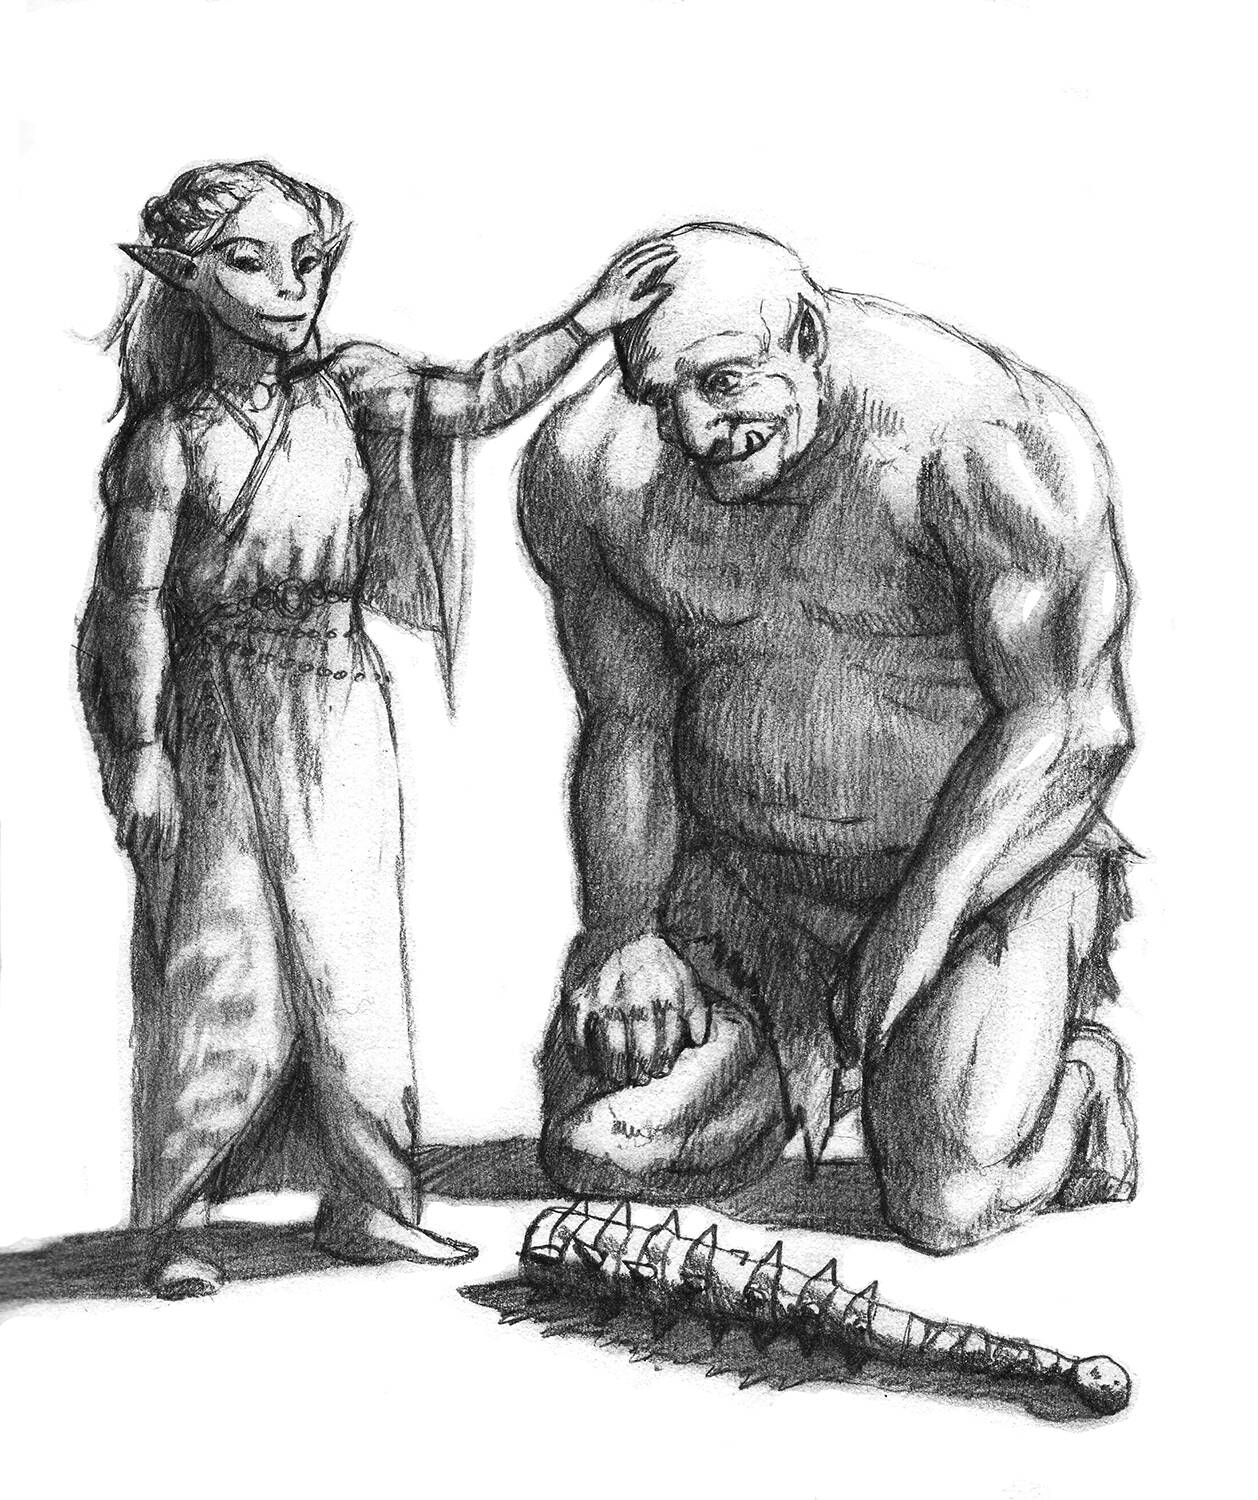
\includegraphics[width=.43\textwidth]{images/Roch_Hercka/elvish_enchanter.jpg}
	\label{roch:enchanter}
}{}

At the end of the scene, targets make one final resisted roll against the enchanter's Intelligence + Deceit (even if the enchanter is no longer present). Failure indicates that the target has forgotten the encounter entirely, including some moments before when the spell began.

If an \gls{npc} enchanter intends to cast this on a \gls{pc} during a scene, the \gls{gm} is encouraged to simply make the resisted roll for the spell.
If the player fails the roll then the \gls{gm} can infer what probably would have happened had the scene played out and skip to the next scene, telling the player that something important might have happened, but that they cannot remember any of it.

When this spell hits someone out of combat, perhaps during a conversation, targets tend to flap their mouths open and shut like a confused fish as they try to recapture their train of thought. The use of magic will is not obvious to those unfamiliar with such abilities.

\spell{Mind of Stone}{Continuous}{Empathy}\\
Enchanters of this level can also cast a greater version of Mind's Healing. The spell can cut the ill effects of any Enchantment spell and if cast as a standing spell the target becomes completely immune to unwanted Enchantment spells.

\spelllevel

The enchanter locks eyes or otherwise engages with the target and lulls them gently to sleep, forces them to repeat particular actions, or fills them with a dreadful fear. The target can reroll a failed resistance roll at the end of each scene.

\spell{Focus}{Continuous}{Empathy}\\
The target holds the last action performed and repeats it, again and again.
If they were attacking, they will continue attacking until there are no targets left, and then go and look for more.
If the target was attempting to mount a horse but the horse flees, they will chase it until they can no longer move.

The enchanter engages in a resisted roll of their Intelligence + Empathy versus the target's Wits + Academics.
Targets can stop once their original action has become obviously impossible or is unmistakably complete.

\spell{Panic}{Continuous}{Deceit}\\
The enchanter and the target make a resisted roll; the caster adds their Intelligence Bonus and Deceit Skill while the target adds their Wits Bonus and Combat Skill. If the target fails, they automatically run away in fear, as the enchanter dictates.

If the target would normally take a Morale Check, the caster's Intelligence + Deceit are added to the \gls{tn} for as long as the spell is in effect.
Targets completely unable to flee can continue to fight.

\spell{Sleep}{Continuous}{Empathy}\\
Enchanters who want their target to fall asleep can make a resisted Intelligence + Empathy roll against the target's Wits + Academics.
The target can spend 5 \gls{fp} to ignore the results of the spell. A successful spell means that the target has fallen asleep.

\spell{Expectations}{Continuous}{Varies}\\
The caster can make someone believe something they were already expecting to see.
If they thought they had beer in their cup, they will continue to drink it, even when it's been replaced by something else.
If they expected to see a dragon in a cavern, they will walk round a corner and believe they are face to face with a dragon.

The caster might look deeply into the target's eyes and force them to hear music which is not in fact there but persists despite all attempt to stop it. They might sing to all present about a dragon, and one particular listener will actually see, feel and smell that dragon.

In all cases a successful illusion will be complete, and the target will make every provision to interact realistically with the imaginary thing, be it a creature, an object or weather condition. It could even be something stranger, such as a box containing a spider's voice, or a statue of a sunrise which glows in unknown colours.

The caster and target make a resisted roll: the caster uses their Intelligence + some Skill relevant to the illusion being created. A caster making a dragon might use Ether Lore, while making an illusory cow would require Beast Ken. The target resists with their Wits and the same Skill as the caster.

The \gls{gm} should make this roll for players, in secret. The target gains a bonus to resist (or the caster takes a penalty) if the illusion is particularly unbelievable (such as a bizarre object or an unexplained dragon). Targets also gain a penalty to resist if they suspect that magic is being used to trick them, which often becomes obvious if lots of people around are insisting that rats are not in fact biting off their toes.

Such mental illusions can inflict up to 4 Fatigue Points plus the caster's Intelligence Bonus and multiple castings allow the Fatigue Points to stack up. These Fatigue Points are healed as normal. The player may be told that this is Damage, but the \gls{gm} should keep track of it separately to ensure that all the Damage is properly converted once the spell fails. Such Fatigue Points can kill a character in the usual manner, i.e. by giving the target a Fatigue Penalty beyond -5.

\spelllevel

\spell{Domination}{Continuous}{Deceit}\\
The target is given a simple command by the enchanter, consisting of no more words than \arabic{spelllevel} plus the enchanter's Intelligence + Deceit. If the target fails the resisted task of their Wits + Academics against the enchanter's Intelligence + Deceit then they must immediately obey any commands the enchanter gives them.

If the enchanter maintains the spell then the target can reroll at the beginning of each scene to break the spell again, otherwise it ends when the enchanter drops the spell.

\end{multicols}

	\begin{tcolorbox}[arc=1mm,tabularx={llp{.5\textwidth}}]
		Task Bonus & \gls{tn} & \\\hline

		Humiliation & +2 & Any action which would humiliate the target grants a +2 bonus to resist. \\

		Betrayal & +4 & Targets who would otherwise be weak-willed and at the mercy of the enchanter gain a +4 bonus to resist attacking their allies. This bonus can increase up to +6 to resist attacking loved ones such as family and close friends.\\

		Code Violation & Variable & Targets forced to act against their own code or god gain an additional bonus to act equal to the amount of \gls{xp} they would receive for completing the action.
	For example, those following the code of passion would gain 1\gls{xp} for trying a new type of food or drink, so they gain a +1 bonus to resist commands which inhibit their ability to act in this way.
	Those following \gls{wargod} gain 10 \glspl{xp} for bringing down a sufficiently large monster, so they would gain a +10 bonus to resist any enchantment which prohibits them from slaying such quarry.
	This can also be used against the target, with the enchanter gaining a bonus to affect someone with an order if it adheres to the target's code.
\

	\end{tcolorbox}

\begin{multicols}{2}

\noindent
Giving a command can take some time, so in combat, Enchanters have to spend the usual 2 Initiative to speak in order to actually make a target do something, once the spell has been cast.

Some commands are easier to resist than others. Particularly repugnant commands allow the target to reroll to break the spell with a bonus.

\spelllevel

\spell{Mental Bondage}{Continuous}{Deceit}\\
The enchanter locks down the target's every thought and turns everything they know to a desire to serve only the enchanter. They will follow any command to the best of their abilities, and if asked why will proclaim an unconditional love for or obedience to the caster.

The target makes a resisted task of their Wits + Academics against the enchanter's Intelligence + Deceit.
Success (from the target's point of view) means that the target breaks the spell but failure (a successful roll on the part of the enchanter) means that the spell is fixed -- for as long as the caster wishes the target will serve them loyally.
Immediate threats to the target's life, such as being told to jump off a cliff or being told to drink something by an enchanter who was previously trying to kill the target call for a reroll, but there is no automatic reroll at the beginning of each scene.
This spell is subject to the same modifiers as the previous level.

Enchanters might use this to turn attacking ogres into a loyal group of warriors to use against other enemies, or simply to turn a favoured artist into a persistent plaything of the local court. This spell may be expensive in terms of \gls{mp} but over time the target may come to loyally serve the enchanter naturally, assimilating the spell into normal, everyday habits. Every month of service prompts a new roll -- success means that nothing happens while if the target fails they must serve the enchanter even after the spell has been cancelled, with full normal effects. Enchanters do not know when their spells have turned into long-term spells, but they can often guess by looking at just when the target has stopped trying to fight the spell.

If the enchanter ever dies, the target can reroll each scene to break the spell.

\spell{Tabula Rasa}{Continuous}{Deceit}\\
The target's memories can be filched -- either selectively or not. The caster specifies (through song, words, or a simple glance) which memories are to be removed. If a target loses access to a Skill due to this spell, they can no longer use it until the spell ends.

The caster uses their Intelligence + Deceit while the target resists with their Wits + Academics.
Success means that the caster has free reign, not to rifle through the target's exact memories, but to specify that anything they wish is lost, up to and including all memories.
The target always retains their first language.

\end{multicols}

\sphere{Fate}
\index{Magic!Fate}Fate deals with divine blessings and luck. At first the caster learns to ask questions of the gods, or to perhaps reach into an inner intuition about the world. Next up the mage learns to heal people's \gls{fp} and increase targets' average luck. Finally, priests can help bring people back from the edges of death.

\begin{multicols}{2}

\spelllevel

\spell{Curse}{Continuous \& Instant}{Deceit}\\
Additionally, casters can curse a target. The target loses $1D6$ \gls{fp} plus the caster's Intelligence Bonus. If the target has no \gls{fp} then this spell has no effect. The mage is allowed to know how many \gls{fp} the target has lost. The target cannot dodge in any way -- the caster simply rolls their Intelligence + Deceit against \gls{tn} 7.

If cast as a standing spell, the target's \gls{fp} are reduced by the spell's level plus the mage's Intelligence Bonus for as long as the spell endures.

\spell{Eyes of Fate}{Continuous}{Empathy}\\
The priest prays for guidance, gains a keen insight into the fate of others.
Once the spell is cast, the priest knows the current \gls{fp} of the target.

This spell grants total immunity to the Enchantment spell, \textit{Fear}.

\spell{Intuition}{Instant}{Varies}\\
When players search for an item, or ask around town for someone's whereabouts, the \gls{gm} often won't tell them the \gls{tn}.  With this spell, the priest may demand to know the \gls{tn}.  The Skill used is the same as that being used in the task, so asking about a roll for Crafts means using the Crafts Skill for the spell.

\spell{Lending Hand}{Continuous}{Empathy}\\
The priest blesses a target with +1 to any Skill, so long as the priest has a higher level than the target in that Skill.

\spelllevel

\spell{Auguary}{Instant}{Academics}\\
The character requests guidance about the future and receives a cryptic message from their deity, from dreams, or simply the shape of nearby clouds.

The \gls{gm} should roll for the player so the player is unsure how accurate the information is.

The \gls{gm} might create some riddle, or describe a prophetic vision.
Alternatively, if the Encounters or Side Quests systems are being used, the \gls{gm} may choose to describe an upcoming encounter or read out upcoming boxtext.\iftoggle{verbose}{\footnote{See pages \pageref{encounters} and \pageref{sidequests} respectively.}}{}
If it succeeds, boxtext or encounters can be taken from a different area, or a later encounter.
And if the roll succeeds with a Margin of 4 or more, the player can elect a specific area to receive the boxtext from.
If the roll fails, the \gls{gm} can create misleading information.

If the party radically change their plans in order to avoid an encounter they think sounds bad, the Side Quests should be randomized, leaving some chance they will encounter the same place again.

Characters who continue to cast Auguary receive the same answer each time until they have run into the encounter, or somehow bypassed it.

Nobody with this power ever says ``you cannot change your fate''.  Changing your fate is the entire point of this spell.  Besides, if the spell ever appears to go wrong, the local priests will explain that it actually predicted events correctly.  It was simply your knowledge of the spell that -- somehow or other -- altered what would otherwise have been a fine prediction.

\spell{Blessing}{Instant}{Academics}\\
The priest blesses the target with the favour of the gods. The target `heals' or regenerates $1D6$ \gls{fp} plus the priest's Intelligence Bonus. This cannot take the target above their maximum \gls{fp} score.

\enhancement{1}{Generous}
\index{Spell Enhancements!Generous}

The priest heals the target for an additional 2 \gls{fp}.  These \gls{fp} stack just like Damage, so $1D6+4$ \gls{fp} becomes $2D6$ \gls{fp}.

\spelllevel

\spell{Fortune}{Continuous}{Empathy}\\
The priest blesses a target, who then receives a +1 to any Skill.
This does not stack with any other Fate spells.
This spell can take a character beyond the standard Skill levels.

\spell{Prayer of Gratitude}{Instant}{Academics}
The caster rolls during any scene in which someone spends at least 2 Story Points.  With a successful roll, one Story Point is returned to the character.

\spelllevel

\spell{God's Chosen}{Continuous}{Academics}\\
The target increases their maximum \glspl{fp} by a number equal to the spell's level, plus the caster's Intelligence Bonus.
The character instantly heals a number of \glspl{fp} equal to $2D6$ plus the caster's Intelligence Bonus.
When the spell ends, the maximum FP return to normal.
The spell does not increase the rate at which FP are regenerated.

\spelllevel

\spell{Divine Favour}{Instant}{Academics}\\
The priest spends 1 Story Point and gains an addtional 5 Story Points plus their Intelligence Bonus, which must be spent immediately.  This can be used on a summoning miraculous help, such as a crew of soldiers who have a debt to the priest, or a magical ally.\footnote{As usual \gls{gm} is free to veto any ideas, but the player is also free to continue pulling new ideas out.}

\spell{Resurrection}{Instant}{Medicine}\\
The priest summons the soul of a recently deceased person back to their body. If they are beyond -3 Hit Points, they must roll a Vitality Check again to stay alive, but this time with a +5 bonus. There is no roll for the caster -- the spell is automatic and the spell is instant, so the effects need not be maintained. If the spell is made into a standing spell then the effects count as being continuously cast.

The spell also heals the target of a number of \gls{hp} equal to half the Margin.
This cannot bring the target above 0 \gls{hp}.
For example, if a \gls{pc} were at -7 \gls{hp} they would normally make a Vitality Check at \gls{tn} 11.
Adding in the Bonus would make the adjusted \gls{tn} 6.
If the Vitality Check were a roll of 11 then the Margin would be 5 and the character would heal 3 \gls{hp}, going up to -4 \glspl{hp}.
This healing should be understood as a retroactive blessing from the gods, indicating that the Damage sustained was not nearly so bad as was once thought.

The spell must be cast within the same scene as the target lost their last \gls{hp}.

If cast on a member of the undead, the target loses $2D6$ \gls{hp} plus the caster's Intelligence Bonus.
No roll is made, and no protection can be given from \gls{fp} or \gls{SP}.

\spell{Mana Lake}{Continuous}{Empathy}\\
The priest spends a Story Point to sanctify an area, creating a mana lake.
Forever afterwards, the area spills out mana to be absorbed by anyone nearby with empty mana slots.
The caster rolls at \gls{tn} 12.
Each Margin on the roll means one \glsentrylong{mp} is generated each round, so achieving a `14' on the roll would produce 2 \gls{mp} each round.

\end{multicols}

\sphere{Force}\index{Force}

\begin{multicols}{2}

\noindent
The mage can shape pure energy, pushing and pulling at the world with the power of their will alone. They can create magical shields, pick up weapons and grind targets into the ground as if with an invisible, giant, floating hand.

\spelllevel

\spell{Levitation}{Continuous}{Combat/ Craft}\\
The mage focusses on something and forces it to float in the air.
The caster rolls their Intelligence and Craft Skill against a \gls{tn} of 7 plus the target's \gls{weightrating}.
The spell grants an effective Strength Bonus equal to the level in the Force sphere being used.
Any object with a \gls{weightrating} of up to 4 points higher than this Strength score can be lifted into the air but the heavier something is the slower it will move.

If creatures are targeted for levitation, they have a \gls{weightrating} equal to their \gls{hp} and the mage rolls Intelligence + Combat to lift them.
They can add their Speed Bonus to the spell's \gls{tn} in order to attempt to wriggle free of the telekinetic hold.
Trying to wriggle free takes 2 Initiative points.
Targets can be moved at a Speed rating equal to the level in Force.

Mages attempting to lift people into the air can move the target only at the rate of a standard action -- i.e. 3 squares per turn plus their effective Speed rating.
The effective Speed rating is equal to the spell's level, but the spell can be encumbered just like lifting a normal person.
So casting a spell at level 3 means an effective Strength and Speed rating of 3; if the target had Strength +1 they would have 7 \glspl{hp} and therefore a \gls{weightrating} of 7.
That's 4 points above the spell's rating so the Speed suffers a -4 encumbrance penalty, making the total movement 1 square every two \glspl{round}.
The target could roll to be free every 4 Initiative steps, rolling against the spell's effective Strength Bonus.

While a target is being levitated, they are especially vulnerable to attack, and all attacks against them count as Sneak Attacks, gaining +4 to Strike and +2 to Damage.

\spell{Lock}{Continuous}{Craft}\\
The mage can erect a magical force field, similar to mage armour, over a doorway to make it more difficult to break through.
The \gls{tn} to break through the door increases by an amount equal to double the level of the Force sphere being employed plus the mage's Intelligence Bonus.
For example, if a door were at \gls{tn} 8 to burst through, a mage with Intelligence +2 could cast the second level of the Force sphere, raising the \gls{tn} to 14.

Mages can also create barriers of pure force to block passageways without a door, just as with mage armour.
The blockade has a number of \gls{SP} equal to triple the level of Force sphere being employed plus the mage's Intelligence Bonus and must be battered through with repeated blows to get through the portal.

\spell{Mage Sight}{Continuous}{Vigilance}\\
The mage can `feel' by delicately touching things with mental movement rather than actually seeing them. They can see in complete darkness whether underwater or on land.

The mage rolls Intelligence and Vigilance at \gls{tn} 6 plus the spell's level.
The spell covers a progressively larger area depending upon the level used.

Mages able to perceive events multiple areas away make for legendary spies, although the power is limited by the fact that while the make can feel events at a distance, they cannot hear voices or read anything.

Any two mages `looking' at the same area can feel each other's presence and instantly understand that someone else is using Mage Sight.
They can even identify the other mage with a Wits + Empathy roll.

\spell{Slow Fall}{Continuous \& Instant}{Athletics}\\
When people (or even items) are falling to their doom, force mages can slow the decent, limiting the Damage from such a fall.
The total spell grants a resistance to any Damage incurred through falling equal to 4 points per level of the Force sphere used plus the mage's Intelligence score.
Therefore, a mage with Intelligence +2 using the third level of the Force sphere would subtract 14 from any Damage incurred through falling.

If cast as a Quick Spell, it can be cast as a Quick Action, outside the usual Initiative order.

\spell{Telekinetic Fist}{Continuous}{Combat}\\
The mage uses powerful telekinetic blasts to hold and crumple targets in close combat.
Unarmed attacks using Telekinetic fist count as normal Damage instead of inflicting Fatigue Points.
For the purposes of these attacks, the caster counts as having a Strength Bonus equal to the level of the Force sphere being used.
For example, someone employing the third level of the Force sphere would count as having +3 Strength, and would inflict $1D6+3$ Damage with unarmed attacks.

\spell{Telekinetic Retreat}{Continuous}{Athletics}\\
Mages can add their mental ability to move things to aid their movement.
Any attempts to move, whether fleeing or just flitting around a room, gain a bonus equal to the level of the Force sphere being employed plus their Intelligence Bonus.
The mage can cast the spell on others and it will automatically push them onwards in whichever direction they are running.

\spelllevel

\spell{Dancing Swords}{Continuous}{Combat}\\
The force mage can make a weapon levitate with the power of their mind. It can float nearby to defend them and even float off to stab at enemies who will be hard pushed to counterattack the wielder when they're standing some distance away.

The caster rolls Intelligence + Combat to levitate the weapon.
They gain an effective Strength Bonus for the purposes of wielding the weapon equal to the level of the Force sphere being used minus one.
This must be sufficient to lift the weapon without encumbrance, so a mage casting the first level of the Force sphere would have an effective Strength Bonus of 0 and could wield a dagger.
To wield an axe a mage would have to use the fourth level of the Force sphere, gaining an effective Strength Bonus of +3.

While the weapon is next to the caster it can defend them just as any weapon. An axe would add +1 to the caster's Evasion Bonus while a long sword would add +3 to the caster's Evasion total. The weapon can add this defence to anyone nearby but only one person at a time.

To attack with the weapon, the mage spends the normal amount of Initiative for that weapon; e.g. 4 for a dagger and 6 for a shortsword.
They roll with Intelligence + Combat and deals the normal amount of Damage given the effective Strength Bonus, so a fourth level Force sphere spell could wield a dagger to deal $2D6$ Damage, or could wield an axe to deal $2D6+2$ Damage.

If the mage levitates multiple weapons (through multiple castings or casting a \textit{Wide} spell), each additional weapon adds +1 to their Strike score, adds +1 Damage and +1 to the Evasion Bonus.\footnote{Casting over a massive number of weapons works fine, but the mage cannot direct all weapons properly at the same time, so the maximum number of weapons in use is always equal to the spell's level plus the caster's Wits Bonus.}
In this way the mage can add up to a maximum of +3 to each stat, meaning only the first four weapons can have an effect.
Additional weapons can add Evasion Bonuses behind or to the side of the mage to ensure they do not lose any Evasion Bonus when attacked from behind but a fifth weapon cannot add additional Damage.

If someone wants to grab one of the floating weapons they must roll with their Strike Factor just as when making a grab against any character.
The mage defends with their normal Evasion Factor and a successful grab means that the weapon has been arrested.
The weapon gains a \gls{weightrating} equal to the Weight of the character grabbing the weapon (which is equal to their maximum \gls{hp}).
At this point the weapon is too heavy to lift and the spell ends.

The levitated weapons do not add a Speed Bonus to the caster's Initiative -- they must use their Wits Bonus as usual.

The caster may not employ any special combat manoeuvres such as pushing people back or fighting in the Aggressive Stance. No Knacks concerned with Combat apply to the mage wielding such weapons.

Mages who must slowly cast a spell can still weild weapons instantly.  Runecasters might require a full scene to make a dagger float, but the floating dagger can thereafter be used to attack or even defend at the normal Initiative rate.

\spell{Mage Armour}{Continuous}{Academics}\\
The mage casts a shield of crackling energy around the target to protect from all harm, and most often mages target themselves.  The barrier can shatter if attacked but can take a serious beating before breaking. Each barrier counts as a having a number of \index{Shield Points}\gls{SP}, which are destroyed by Damage like \gls{fp}, but always before \gls{fp} are targeted.
The target gains a number of \gls{SP} equal to the level of spell used times 3 plus their Intelligence Bonus.

Those protected by the shield cannot attack others as the shield stops all attacks.
However, casters are able to focus enough to use missile weapons and spells by allowing small breaches in the shield's wall.
\footnote{Allowing a target to use a missile weapon requies complete focus, and a Wits + Empathy roll, and can be performed as a Quick action, costing 2 Initiative Points.}

The shields cannot `split' into bubbles.
When cast wide, it can cover a group of people, but the shield will cover all of them or none.

\textit{For example, Annabel the alchemist has the Force sphere at level 3 and Intelligence +2.
She's low on \gls{mp} so she casts it at level 2, gaining 8 \gls{SP}.
On the very next Initiative Count she's hit for 10 Damage and loses all 8 \gls{SP} then 2 FP.}

The spell must be maintained as a standing spell to function. Multiple castings do not stack -- only the highest casting it used. The shield can be placed on others if need be, not only the mage.

Armour does not block Damage going onto \gls{SP} -- the character simply subtracts \gls{SP} without any \gls{dr}. The Mage Armour is not affected by a Vitals Shot -- it protects all around, counting as Perfect armour, although not quite continuously enough to keep out water or gasses. Multiples of such spells do not stack -- only the highest is used.

\spelllevel

\spell{Telekinetic Grasp}{Continuous}{Combat}\\
Force mages can wrestle with people from afar using telekinesis. One major advantage with this sort of wrestling is that the mage does not risk being hit back as they can cast the spell from afar. As per the Grappling rules, the mage first makes a roll to capture the target; they roll Intelligence and Combat while the target resists with their current Evasion Factor. Targets can literally feel the force of the mage's mind around them, often described as a hundred tiny, invisible hands or the feeling of an invisible wave. This force can be parried and pushed back like any normal weapon, so targets can use their full Evasion Factor, including bonuses from using a weapon.

If the spell is successful, it inflicts no Damage nor Fatigue Points, but the target counts as carrying an item with a \gls{weightrating} equal to the level of the Force sphere being used.

For example, a mage using Force level 2, with Intelligence +1 and a Combat Skill of +1, could cast Telekinetic Grasp on a gnome.
The gnome adds their Evasion Factor to the basic \gls{tn} of 7 and then the mage resists this with their Intelligence Bonus plus Combat Skill.
If successful, the gnome would count as carrying an item with a \gls{weightrating} of 2.
Assuming this gnome has the usual Strength Bonus of -2, they would then receive a -4 penalty to their effective Speed Bonus.
Their Initiative Score would suffer and they would accrue additional Fatigue Points each time they attempted to run or fight due to the added \gls{weightrating}.

When cast over a full area, all are effected, and movement becomes extremely difficult.



\end{multicols}

\sphere{Illusion}\index{Illusion}

\begin{multicols}{2}

\noindent
Illusions create a facsimile of sounds and sights out of pure magic. The thing created might look like a hat, a coin, a rat or even a dragon at higher levels. Illusions also create convincing sound -- loud echoes, the sound of nearby battle, perhaps even imitating an enemy commander's orders in battle. However, illusions are little more than coloured air and noise -- once touched they fade away. They are frightening and if properly used can defeat armies, but are not perfect weapons by any means.

Seeing through an illusion is always an opposed roll -- the victim uses Wits + Vigilance, while the Illusionist uses Intelligence + some appropriate Skill.
If a \gls{pc} could be tricked by an illusion, the \gls{gm} should always roll for the illusionist, without informing the players.
If someone has a reason to suspect that something is an illusion, they should receive a +2 bonus to resist it.
The party also receive a bonus for multiple people who might spot the illusion, as per the standard Vigilance Skill rules.

Illusionists add different Skills to the roll, depending upon what they are making an illusion of. An illusion of a cart or sword might require the Craft Skill. An illusion of a monster might use the Academics Skill. Specialisations in the correct area are, as usual, a requirement if the caster wants to avoid the usual -1 penalty for lacking the appropriate specialisation.

For example, a gnome creates an illusion of a fleeing gnoll with a great bundle of treasure in his hand, hoping the \glspl{pc} will chase after him immediately.
His Intelligence is +2 and his Academics is at +1 though he has no appropriate specialisations, so the players are rolling at \gls{tn} 9.
The \gls{gm} takes the party member with the highest Wits + Vigilance who has a score of +3 in total.
The next highest score in the party is +2 but nobody else has anything to contribute.
The total is +4\footnote{See the rules on teamwork, page \pageref{teamwork}.} so the \gls{gm} rolls for them and obtains a total of 8 -- that's not enough.
As they begin to run, one of the \glspl{pc} remembers they heard about a gnomish illusionist and asks `Are we chasing an illusion?' -- that puts that final score up to 10; the \gls{tn} is reached and the \gls{gm} informs the player that she sees that the gnoll's feet are not always touching the ground properly, so it must be an illusion.

The \gls{gm} should grant bonuses and penalties to illusions depending upon lighting conditions -- illusions inside a shadowy cottage seen from far away should receive an immense bonus, while far-fetched illusions on a sunny day seen up close might receive a penalty.

Illusionists typically create images of things they are familiar with. Unfamiliar objects, such as an illusionist trying to recreate a dragon while never having seen a dragon, suffer a -2 penalty to the roll, at minimum.

While most people are aware that illusion magic exists and so are suspicious of anything outlandish or out of the ordinary, those who have never heard about illusory magics suffer a -2 penalty to disbelieve.

If someone sees an illusion for what it is then the illusion remains, but of course will have less effect. However, while someone fully believes an illusion to be real, they can be psychosomatically damaged by it simply by believing that it's real. All illusions can inflict a total of 1 Fatigue Point per level of the illusion spell plus one per Intelligence Bonus of the caster. For example, a song mage might sing a griffin illusion into existence; all who are fooled by the illusion can be `attacked' by it, receiving up to 4 Fatigue Points. On later \glspl{round} the song causes no more Fatigue Points, even if it keeps playing, but the bard could then create the illusion of a sword using the first level of the illusion sphere. They could use the sword to attack as usual, but not parry blows. While attacking, they could inflict up to 2 Fatigue Points as people believe they have been wounded by the sword, but subsequent attacks would not increase the amount of Damage.

Illusions must be summoned within the normal range of spells, but once summoned they can travel away from the caster without worry -- so long as they are maintained as standing spells, they endure, no matter how far away the caster might be.

\spelllevel

\iftoggle{verbose}{
	\noindent\includegraphics[width=\linewidth]{images/Roch_Hercka/illusion_trogdor.jpg}
	\label{roch:light}
}{}

\spell{Illusion}{Continuous}{Varies}\\
The illusionist can make anything look like another of roughly the same size.  A fox can look like a dog, a copper coin can look golden, or a gnome can appear like a gnoll.

Illusionists can use this to hide by making themselves look like a bush, or slip unseen into a party by making themselves look like one of the other guests.

Copying a person requires the Empathy skill, while copying furniture would require the Crafts skill.

Anyone touching an illusion finds that it melts in their hands -- a simple handshake can shatter a basic illusion, and handling fake coins quickly dissipates the magic.

Illusionists cover both sound and appearance.  Illusions crafted for sound can change a nearby river to sound like howling wolves, or make someone's voice come out high-pitched.

Illusionists who speak another language can make someone else's speech sound like that language.
If you speak gnomish, your colleagues can be made to sound like they speak gnomish.
Another spell could make a number of gnomes sound like they're speaking in the common tongue.\footnote{Of course at that point, everyone would understand each other, but have a hard time understanding themselves.}

Seeing through an illusion requires a Wits + Vigilance roll, with a \gls{tn} equal to 7 plus the caster's Intelligence and skill (whatever it happens to be).  Alternatively, when a player rolls for an illusion, the \gls{tn} is 7 plus an opponent's Wits + Vigilance.  Having multiple \glspl{tn} can mean some opponents are fooled and some are not.  Anyone specifically looking out for an illusion can gain a +2 Bonus on the roll, or a +4 if they have reason to suspect that the thing in front of them is an illusion.

Illusions require a caste's full focus in order to remain realistic.  A caster who make his friend look like an elf would have to pay attention to his friend to make sure the facial movements followed along.  Casters cannot engage in anything more than simple conversation or walking while maintaining illusions.

Illusions can only adjust something's size so much.
Something's \gls{weightrating} can increase or decrease by a number equal to the spell level plus the caster's Intelligence.
A first level Illusion spell cast with Intelligence +1 could make an elf look like a gnoll, but could not make a gnome look like an ogre.
Similarly, a shortsword could be made to look like a simple dagger, but turning a chainmail suit into a small bird would extremely difficult.

\spell{Light}{Continuous}{Survival}\\
This replicates the Aldaron spell, \textit{Light}, page \pageref{light}.

\enhancement{1}{Independent}
\index{Spell Enhancements!Independent}

Illusions can now be cast without any `base' -- they simply appear on their own.
Coins, dogs, dragons, or more, can be fashioned from nothing.
Independent illusions can continue acting in an intelligent manner without any intervention from the caster.
People's speech can be adjusted to another language long after the illusionist has left, or a rock made to look like a human soldier could continue moving and speaking.

\enhancement{1}{Solid}
\index{Spell Enhancements!Solid}

Solid illusions are not all that solid, but they can be touched without disipating and hold all manner of nice details, such as \emph{smelling} right, or stopping smoke from blowing through them.  They are also far more realistic, and increase the \gls{tn} to see through the illusion by 2.

These illusions have a Strength score equal to -5, plus the spell's level, plus the caster's Intelligence and skill.

Solid illusions become an extension of the caster, and any caster can cast a spell \textit{through} the illusion, as if the illusion were the caster.  This might be used to cast an Invocation spell through a dragon illusion, or could employ Force to help an illusory creature lift a sword.

Once even a single point of Damage has been dealt to the illusion, it vanishes.

\enhancement{2}{Negative}
\index{Spell Enhancements!Negative}

The illusionist finally learns to make less of something, rather than more.  A single person can be silenced, or made invisible (or both).

As usual, the illusion is still delicate, and if the person is struck or disturbed in any way, the illusion dissipates.  Combat rolls, for defence or attack, always break such spells unless they are also make \textit{Solid}.

\end{multicols}

\sphere{Invocation}\index{Invocation}

\begin{multicols}{2}

\noindent
This is the first choice of spheres for any battle-mage.
It is designed specifically to destroy targets with balls of lightning and fire.
It also has more subtle uses as casters can extinguish flames, plunging people into darkness.

Armour functions as normal with Invocation, though like any other projectiles, bolts of fire can attain a Vitals Shot (see page \pageref{vitals}) and bypass armour entirely.

All Invocation spells are rolled as Projectiles, using the mage's Intelligence Bonus and their Projectiles Skill;
casters must have a Projectiles specialisation in Invocation or receive a -1 penalty to all spells.
The basic \gls{tn} is 7 and the difficulty raises by +1 for every 5 squares away the opponent is, just as with normal missile weapons.
As usual, opponents who are keeping edgy (see page \pageref{edgy}) can use their Speed to resist the attack, adding it to the \gls{tn}.
Alternatively, if a player is keeping edgy, it is they who can attempt to dodge the incoming attack, rolling their Speed at \gls{tn} 7 plus the pyromancer's Intelligence and Projectiles Skill.
Shields' Evasion Bonus can add to the roll to resist such spells.

Just like any other long-range spell, Fireballs and other Invocation spells can succeed in Vitals Shot, bypassing armour, if they strike precisely enough (see page \pageref{vitals}).
Blast-radius spells such as a \textit{Wide Fireball} can inflict a Vitals Shot on up to 1 person, specified by the caster, but not more as the mage cannot make precise attacks against a group of people simultaneously.

\spelllevel

\spell{Fireball}{Instant}{Projectiles}\\
The mage throws out a ball of flaming, crackling light which strikes and burns the target. The Damage is $1D6$ plus the caster's Intelligence.

\subsubsection{Spell Enhancements}

\enhancement{1}{Raging}
\index{Spell Enhancements!Raging}
The caster increases the spell's level by one and increases the spell's Damage by 2.  A mage with Intelligence +2, casting Fireball at third level would deal $2D6+2$ Damage.

\enhancement{2}{Internal}
\index{Spell Enhancements!Internal}
The pyromancer finally learns how to summon fire upon a target without throwing it -- no ball of flame is thrown, fire simply appears, surrounding the target and instantly covers a target anywhere within normal range. It seeps into soft spots and gets into the chinks in armour, bypassing \gls{dr} entirely, including Perfect armour such as \gls{SP} from Mage Armour. The target cannot resist in any way.

If cast with the \textit{Wide} or \textit{Massive} enhancement, the spell targets everyone inside the area.

\end{multicols}

\sphere{Metamagic}

\begin{multicols}{2}

\index{Metamagic}

\noindent
Metamagic allows the \gls{miracleworker} to enhance their other magic spheres -- adding to their range, casting more spells in a \gls{round}, gaining more \gls{mp} to power them and eventually includes the ability to create magical items.

Metamagic spell enhancements are special.
They can be used to enhance \emph{any} spell from any other sphere.

When Metamagic is used to create magical items by imbuing spells, spells come out in the same way they were put in.
If a spell was cast as a quick spell, it comes out instantly.
It it was cast as a ritual spell, it takes a full scene to take effect.

Magical items always cast spells with the Traits of their casters.
Someone creating an item which raises people from the dead will have a magical item with the same effective Intelligence, Wits and Academics as the caster.

\spelllevel

\spell{Detect Mana}{Instant}{Empathy}\\
The mage casts the spell on any person or item and finds out how many \glsentrylongpl{mp} the target has, including any mana stones the target has.

\spell{Spell Breaking}{Instant}{Sphere Rating}\\
The caster can destroy an existing spell, whether that spell is a persistent effect, such as a Polymorph, or a magical item.
The spell requires an opposed roll of Intelligence + the sphere being used.
For example, a priest casts an Aldaron spell.
She has Intelligence +2 and Aldaron 3.
The \gls{tn} is therefore ($7+2+3=$) 12.
Later, an alchemist attempts to dispel the magic.
He rolls with his Intelligence Bonus of +3, but he does not have the Aldaron sphere, so he can add nothing more.
If he fails the roll, he can attempt to try again, turning this into a ritual spell.
However, if that fails, he simply cannot roll again.

\enhancement{1}{Ranged}
\index{Spell Enhancements!Ranged}

Any spell, from any sphere, can be targeted anywhere the mage can clearly sense, breaking all the normal range boundaries of spells.

\spell{Mana Stones}{Continuous}{Academics}\\
A mana stone is an item which stores mana, and each path of magic has its own version.\footnote{See page \pageref{magic_paths} for more on Paths of Magic.}
Once an item (or creature) is designated as a mana stone, the spell is cast and the mage forfeits any number of \gls{mp} from their maximum.
For each \gls{mp} forfeited, the mage can store 2 \gls{mp} in the stone.
These stones always start life empty, but regenerate 2 \gls{mp} per scene until they reach their maximum.
Anyone on the same Path of Magic can retrieve the mana from the stone by simply touching it and concentrating.
The spell is always permanent -- no additional mana must be kept aside so that the spell remains active.
Retrieving the mana takes the normal amount of time to use an item -- 8 Initiative points

The mana in mana stones cannot be used to create more mana stones and mages cannot enter their own temporary \gls{mp} into the mana stone.

Mana stones form the basis of all magical items, and \glspl{miracleworker} can only use their traditional mana stones to create magical items.

\spelllevel

\spell{Pocket Spell}{Continuous}{Crafts}\\
Pocket Spell is cast on an item to implant a second spell.
Both spells must be cast in succession.\footnote{The magic cannot regenerate mana between casting spells, but can use mana stones while casting a ritual spell in order to gain more mana.}

Some mages create scrolls which are destroyed once read.  Some priests of \gls{naturegod} enchant animals with a single spell, just to see how the animal will use it.
The only limitation is that the mana stone must have enough \gls{mp} to cast the spell once.

The pocket spell always produces a single effect.
The mage can create an item which casts an illusion of a dragon, but never a scroll where the user determines the illusion cast.
Any continuous effects last for \arabic{spelllevel} scenes plus the caster's Wits Bonus.

These magical items are activated by a `command word'.
Command words do not necessarily have to be actual words -- they could be entire phrases or gestures.
Importantly, when activating an item people must spend the usual 8 Initiative points for using an item, because some concentration is always required.\footnote{Knacks cannot reduce this cost.}
Once a spell has started, it cannot be stopped except by counter-spells, even by the original mage who crafted the item.

\enhancement{2}{Mirrored}
\index{Spell Enhancements!Mirrored}

This Metamagic enhancement allows \emph{any} spell be be doubled at the cost of raising it by 2 levels.
A fireball could turn into two fireballs.
An illusion could disguise two people instead of one.

In each case the spell must have different targets, because two copies targeting the same person, would just result in one spell.

\spelllevel

\spell{Magical Item}{Continuous}{Academics}\\
The mage takes a mana stone and allows it to cast a spell, forging a new magical item. A sword could be made which can summon blinding light, or a ruby could be infused with the power to teleport the caster to a nearby location.

Just as with Pocket Spell, above, the mage casts Magical Item and the spell to be implanted in succession, while also relinquishing a number of \gls{mp}.
Any number of spells can be cast into the item, so long as each one is implanted within the same casting.

Magical items function as mana stones and continue to store \gls{mp} for use by people on that Path of Magic.
However, each spell cast into the item lowers the item's \gls{mp} by one.

Such basic spells always take effect in exactly the same way and use the mage's stats for any rolls. A second level Aldaron spell set to freeze water will always do just that, and can never cast a Sunray. An illusion-generating mask, making the wearer into a bush, will always turn that wearer into a bush, regardless of what the user may want the illusion to be of.

Magical items which do not have enough mana simply fail to cast. The one exception here is the Path of Song, wherein spell-songs which have too much mana drawn from them simply break.

\spelllevel

\spell{Greater Item}{Instant}{Academics}\\
This functions just like the Magical Item spell, except that the mage can imbue a full sphere's level.
If the item has Necromancy level 2, it can cast any Necromancy spell of level 2 or less.
If it has Invocation level 3, it can cast any spell at level 3 or less.
Each sphere (but not each level) reduces the item's \gls{mp} by 1.

\enhancement{1}{Sentient}
\index{Spell Enhancements!Sentient}

The mage can make any spell gain some measure of sentience.
Typically, this is made to allow magical items to activate upon a condition, such as a door which turns from solid stone back to wood once the password is stated.

The item acts upon its own Initiative score, and uses the mage's Wits score as its Initiative Factor.
Such items are never capable of a conversation - they only have enough instinct to carry out a single well-defined function.

\enhancement{2}{Forked}
\index{Spell Enhancements!Forked}

\emph{Any} spell, whether Metamagic or otherwise, can now be cast at two levels higher, and gets a number of copies equal to the spell's level plus the mage's Wits.

As with the Mirror enhancement, above, each spell must select a different target.

\spelllevel

\enhancement{1}{Potent}
\index{Spell Enhancements!Potent}

Magical items and stones cast with this enhancement store 3 \gls{mp} per point sacrificed and regenerate 3 \gls{mp} per round.

\end{multicols}

\sphere{Necromancy}\index{Necromancy}

\begin{multicols}{2}

\noindent
Necromancers summon souls from distant, black realms and place them in appropriate bodies -- those of the once living and now dead. The corpses are sometimes filled with their old hosts, locking people into a state of permanent semi-death, or more often with ravenous and malicious spirits from foreign realms. Mages of this sphere begin by imitating the dead, becoming half dead themselves, which allows them to dissuade malicious spirits from attacking.

\spelllevel

\spell{Preservation}{Instant}{Survival}\\
Trainee artists and necromancers have one thing in common -- fruit.
Students of Necromancy often begin their journey by stopping food from degrading.
This spell gives a sort of `half-life' to rot, such that any foods affected slow their own aging process incrementally.
They're not sustained in perfect condition forever, but never quite reach an entirely spoiled stage.

\spell{Torpor}{Continuous}{Medicine}\\
The targed enters an eltered state of semi-death. They ignore all Fatigue Point penalties (but can still become suddenly unconscious due to too many Fatigue Points).
They gain a natural \gls{dr} of 1 which is cumulative with armour -- their corpse-like body bleeds less and feels little pain, only bare sensations written in the mind as cold information.
While this spell is active, no undead will be able to feed from them and most will therefore not wish to attack them.
While this spell is active, the target suffers a -2 penalty to all Charisma checks, though this does not affect \gls{fp}.

This caster rolls Intelligence + Medicine at \gls{tn} 7 to activate this spell. It can never be cast on others. While the spell is in effect they suffer no ill effects from Fatigue Points but cannot heal them. Once the spell is over, the mage often comes crashing down, collapsing from the weight of the awful things they have done to their body while immune to Fatigue. The caster faces a real danger of death if ever they gain enough Fatigue Points to push them over a -5 penalty; they may not gain the penalty but must make a Vitals Check to avoid death and then make another roll each time they gain Fatigue.

\enhancement{1}{Necrotic}
\index{Spell Enhancements!Necrotic}

By adding an additional level to the process, the target can gain the special sight of the undead (in addition to their normal vision).
They can now see all living things, even in the darkness.
Addtionally, the Charisma penalty for the spell raises to -4, as they seem permanently distracted and unable to focus upon the same world that everyone else does.

Additionally, the target's \gls{dr} raises to 2 as the target stops feeling pain altogether.  They can even hold their breath for one minute per spell level.

Targets who die while this spell is in effect raise from the dead as an undead creature.\footnote{This spell cannot raise someone as undead if the necromancer's spell level would not normally allow them to raise a creature of that spell level.}

\spell{Sickness}{Instant}{Medicine}\\
Even low level necromancers have the terrifying ability to pull someone's soul out with a simple spell.  The spell inflicts $1D6-2$ Damage directly to the target's \gls{hp}.  \Glsentrylongpl{fp} and \glsentrylongpl{SP} can be bypassed entirely.  The caster adds their Intelligence Bonus to the Damage.

\enhancement{1}{Fetid}
\index{Spell Enhancements!Fetid}

By adding additional levels, the caster can add 1 \gls{hp} to the total Damage.

\spell{Command the Dead}{Continuous}{Academics}\\
The mage can also command any one undead creature to perform any simple action -- a basic phrase without caveats and no more than one verb.
`Dig',\footnote{The undead are the worst workers due to their stupidity, and typically destroy their own hands before they dig very far.
They can be used for anything, but are not necessarily good for much.}
`kill them all' or `wait here' are all appropriate commands.
To execute the spell, the mage rolls with Intelligence and their Academics score at \gls{tn} 7 -- undead creatures resist with their Wits score, though most have a negative Wits score, which makes resistance difficult.

This spell replicates all five levels of the enchantment sphere with the mage selecting any effect they wish; however, the mage uses Academics instead of any other Skill because the undead may only be `understood' in some technical sense, and not truly empathised with.
The Undead always resist with their Wits + Aggression.

\spelllevel

\spell{Calling the Dead}{Instant}{Medicine}\\
The mage can create their own ghouls from easily accessible realms of malicious spirits. The spell is cast on a small corpse and the corpse is imbued with one such malicious spirit. It retains the Strength score (and therefore \gls{hp}) it had in life.
The corpse has Dexterity, Speed and Wits scores of -2 -- it can run, but not terribly quickly.
The creature has neither Intelligence nor Charisma scores. Most will attack all living things on sight.

The mage rolls their Intelligence + Medicine at \gls{tn} 7 to cast the spell. Any Medicine specialisations dealing with the affected species (e.g. `gnolls', or `humans'), or specialisations concerning death rituals can be used.

At this first level, the mage is limited to fairly small creatures.  The maximum \gls{hp} of the affected creature is equal to 4, plus the mage's Intelligence.  This allows the mage to summon cats, boars, and other animals back from the dead.  More gifted mages might even be able to raise a gnome or even an average human.

Once the spell has been cast, it need not be maintained -- once a soul has inhabited a body it remains there like the permanent resident of a house.

\enhancement{1}{Clever}
\index{Spell Enhancements!Clever}

While the easiest spirits to summon are mindless creatures, more advanced mages can summon smarter creatures.  The creature's basic stats are now Intelligence -2, Wits -2 and Charisma -5.  The mage's Intelligence Bonus, plus each use of this enhancement adds 1 Attribute to the creature's Intelligence and Wits, and 2 levels of any Skill.  Such creatures have a basic mana pool equal to double their Intelligence Bonus.  

For example, a mage with Intelligence +3, using one Clever enhancement, would summon a creature with Intelligence +2, Wits +2, and 4 basic \gls{mp} (6 \gls{mp} in total).

The creatures begin with Intelligence -2, Wits equal to -2 plus $1D6$, and Charisma -5.  For each level of the spell, the mage can add 2 Attribute levels plus their Intelligence Bonus.  An Attribute point can be sacrificed in return for 2 levels in any Skill, or two Attribute points can be sacrified in return for a level in a sphere.

The \gls{tn} is 7 plus one per spell level.  For every margin, the caster can decide where one of the target's Skill points are placed.  The \gls{gm} decides places the rest of the creature's points.

\iftoggle{verbose}{

\begin{exampletext}

	When he was younger, Hugi witnesses his uncle torn apart by a terrible spirit.  His uncle thought to contain it in a small creature, so he summoned the all powerful creature into the body of a little gnome.

	Hugi's uncle, the runecaster, has Intelligence +2, and applies the enhancement twice.  The resulting creature would have Intelligence and Wits at +2, and 8 levels of Skills.  The runecaster rolls a 10, which barely passes the \gls{tn} of 9.  He assigns two of the Skill points to Academics so that he can ask the spirit the question he wants to know.

	The \gls{gm} decides to assign 3 Skill points to Vigilance, 1 to Tactics, and another to Necromancy.

	The result was an uncontainable spirit which cast a death touch spell upon the old runecaster, killing him instantly.

	Hugi decided never to entertain learning necromantic rune magic after that day.

\end{exampletext}
}{}

\enhancement{1}{Greater}
\index{Spell Enhancements!Greater}

With an extra level, the mage can summon the souls of the dead into large creatures.  The maximum \gls{hp} of the target equal to the spell's level times 4 plus the caster's Intelligence Bonus.
A mage with Intelligence +2 could cast Calling the Dead at second level to raise a target with up to 10 \gls{hp}, or at third level for up to 14 \gls{hp}.

\end{multicols}

\sphere{Polymorph}\index{Polymorph}

\begin{multicols}{2}

	\begin{tcolorbox}[arc=1mm,tabularx={XXX}]

	\textbf{Animal} & \textbf{Min Str.} & \textbf{Max Str.} \\\hline

	Cow & 0 & +5 \\

	Badger & -4 & -2 \\

	Basilisk & +5 & +8 \\

	Bear & +4 & +5 \\

	Beaver & -5 & -4 \\

	Bird/ Bat & -5 & -5 \\

	Cat & -5 & -5 \\

	Deer & 0 & +2 \\

	Donkey & 0 & +4 \\

	Frog & -5 & -5 \\

	Goat & -1 & +2 \\

	Griffin & -1 & +2 \\

	Horse & +1 & +4 \\

	Large Cat & +1 & +3 \\

	Pig & 0 & +3 \\

	Rat & -5 & -5 \\

	Wolf & -2 & +1 \\

\end{tcolorbox}

The Polymorph sphere of magic allows the mage to grasp at different strands in the tree of life, and move themselves or others along different paths.  Nearby forms include other races, such as elves turning into men, and later shapeshifters learn to turn into bears, hawks or other animals.  Larger men find it easier to turn into large animals such as griffins, while smaller, lighter people find it easier to take on the form of birds.  Master shapeshifters learn to go beyond the great tree of life and turn into arbitrary forms of their chosing, including living fire, or a gust of wind.

Throughout all these forms people maintain a universal `face' -- a kind of likeness which they simply cannot get rid of.
Many conjecture that the face is a facet of one's soul showing in the world.
A ginger person transformed into a cat would become a ginger cat.
A skinny person with short hair who transforms into a sheep will become a skinny, short-haired sheep.
Spotting someone who has been transformed requires a Wits + Empathy roll, with a \gls{tn} of 8 plus the level of the Polymorph sphere being employed; e.g. if an elf used the first level to transform into a gnome the \gls{tn} would be 9, but if the elf used the fifth level to transform into a magma elemental, the \gls{tn} would be 14.

Unwilling targets who are to be transformed with Polymorph can spend 5 FP in order to retroactively stipulate that the spell fails.  The undead are completely immunte to the Polymorph sphere.

\iftoggle{verbose}{

\begin{exampletext}

	Meldon the elf has 5 \glspl{hp}.
He takes 3 \glspl{hp} Damage and already has 3 Fatigue Points leaving him with a -1 penalty to all actions.
He then transforms himself into a bird, lowering to 2 \glspl{hp}.
He now has zero Damage but retains his -1 penalty due to Fatigue.
After flying away to safety he rests for a while and heals all his Fatigue Points, but when he turns back into an elf all his old wound reappear as his \gls{hp} increases to the point where they can affect him.

\end{exampletext}
}{}

\sidejpg{Roch_Hercka/polymorph.jpg}{
\label{roch:polymorph}}

\noindent
As Polymorph changes people's form it also changes Strength and therefore \gls{hp} maximums.
All \gls{hp} lost to Damage remain as lost \gls{hp} after transformation but might not have any effect.
If a player's maximum \gls{hp} is lowered to the point where they are no longer wounded then all wounds simply vanish, though they are still tracked and reappear once the creature has transformed.
If someone's maximum \gls{hp} increases, once again they count as having lost the same number of \gls{hp}, with no \gls{hp} being gained or lost through the transformation process.
All Fatigue stays where it is and no Fatigue Points which previously gave no penalty move to giving the character a penalty.

The new form granted by a Polymorph spell always feels a little strange, so anyone who transforms suffers a -1 penalty to Dexterity until they get used to the new form.\footnote{Any amount of downtime is a reasonable amount of time.}

Nobody is terribly comfortable holding another creature's form.  Like a newborn lamb, such transformations make people clumsy.

\spelllevel

\spell{Polymorph}{Continuous}{Medicine}

The basic Polymorph spell allows someone to turn into another race, so long as the racial difference in Strength is not greater than the spell's level.
When cast at first level, gnolls can turn into humans, humans can turn into dwarves, dwarves can turn into elves, and elves can turn into gnomes.

Once the change has applied, the original racial Bonuses are discarded, and the new racial bonuses applied.
Gnomes who turn into elves gain +1 Strength and +1 Speed, and dwarves who turn into gnolls gain +1 Strength, +1 Speed, but -1 Dexterity.

Various enhancements allow the spell to be cast at a higher level, meaning a skilled Polymorphing gnome could eventually learn to turn into a gnoll.

Changing one's own form is \gls{tn} 7, while changing another's is \gls{tn} 10.

Polymorphing into another race does not grant any of its racial abilities.
Changing one's shape to look like an elf will not grant cold-immunity, and Polymorphing into a human will not allow one walk long distances without fatigue.

\spell{Animal Transformation}{Continuous}{Beast Ken}\\
This spell allows the mage to transform one animal into another.
An animal is defined as any living creature without an Intelligence Bonus.
As before, the mage can increase or decrease the target's Strength Bonus by the spell level,
but have to keep within the normal size-boundaries of the animal.
If a boar has Strength +1, turning it into a bear will require an additional 3 points of Strength, because bears have a minimum Strength of +4.
If the caster instead tries to turn a dangerous bear into a housecat, this is a prohibitively difficult task, as house cats have a difference of at least 9 levels of Strength.

The \gls{tn} for such a transformation is 12, as understanding how animals function is a serious challenge to those used to walking on two legs.

Such animal transformations are in shape alone, and do not grant any abilities.  Polymorphing into a bird will not let one fly, and taking the shape of a bear will leave a weakened facsimile of the bear's strong teeth and hide.

\enhancement{1}{Bolstered}
\index{Spell Enhancements!Bolstered}

\iftoggle{verbose}{
While basic shapeshifters base their range on the Polymorph spell's level, a \textit{Bolstered} spell allows the caster to use a number of points equal to the spell's level plus their Intelligence Bonus.
If a shapeshifter cast this spell at the second level, with Intelligence +1, they could lower an animal's Strength Bonus by 3, or could turn a human into a gnome, since that requires a Strength adjustment of 3.

Those with the \textit{Realistic} enhancement also gain a number of \textit{Form Points} equal to the spell level plus the caster's Intelligence Bonus, instead of simply gaining points equal to the Spell's level.}{

The caster uses the spell level plus their Intelligence Bonus to determine all facets of the spell's potence, rather than just the spell's level.

}

\enhancement{1}{Empathetic}
\index{Spell Enhancements!Empathetic}

Advanced shapeshifters can extend a little mana into their understanding of alternate forms, and discard the usual \gls{tn} restrictions.  All \glspl{tn} become 7, and the target no longer suffers a Dexterity penalty for transforming.

\enhancement{1}{Realistic}
\index{Spell Enhancements!Realistic}

The \textit{Realistic} enhancement allows mages to take on creatures' natural abilities with a number of \textit{Form Points} equal to the spell's level.  When transforming a target into an animal, the form of a bird can allow the target to fly, the form of a bear includes teeth, claws and a thick hide.

The Form Points can each be spent on one of the following:

\begin{itemize}

	\item{Claws \& Teeth: +1 Damage}
	\item{Flight: The creature has wings, and can use them properly.}
	\item{Thick Hide: The animal's thick skin grants \gls{dr} 2.}
	\item{Underwater Breath}

\end{itemize}

When the target is to transform into an animal, all unused points are applied to the target's Speed Bonus.  Someone transforming into a bird with 3 Form Points could use one to gain realistic flight, and then +2 Speed.

When transforming into another race, the target merely loses their racial ability, and gains any racial abilities of the target which are concerned with the body.  For example, elves who transform into dwarves lose their immunity from natural cold, but gain the dwarvish ability to consume strong drink.

\enhancement{1}{Trans Species}
\index{Spell Enhancements!Trans Species}

The Polymorpher can now cross the species boundary, making themself or another transform entirely into an animal.

Alternatively, the Polymorpher can turn an animal into a person.
This won't yeild any fantastic results, as animals don't suddenly become intelligent once turned into a gnome or dwarf, but it is possible.
Such creatures start with Intelligence -5 and Charisma 0.

This spell is cast at \gls{tn} 12, as it either targets an animal, or makes a person into one.  It uses the Skill associated with the creature the target will become, so turning a wolf into a man uses Medicine, while turning a man into a wolf requires Beast Ken.

\spelllevel

\spell{Freeform}{Continuous}{Ether Lore}\\
The shapeshifter can throw off the limits of existing and known creatures, and turn into flamming bulls, acidic clouds, or anything else they might imagine.  The basic \gls{tn} for the spell is 14 as the alternative forms are alien even to those who are capable of adoptin them, but as usual the \gls{tn} can be reduced by other enhancements.

As with the \textit{Realistic} enhancement, the caster gains a number of Form Points equal to the spell's level.  The caster can spend \textit{2} form points to purchase any of the following:

\begin{itemize}

	\item{Massive Claws \& Teeth: +2 Damage.}
	\item{Impenetrable Hide: +4 \gls{dr}.}
	\item{Etherial Form: The caster turns into a thick smoke or mist, becoming immune to almost all physical damage.}
	\item{Fiery Form: The caster's body is composed mostly of acid, fire, or some other dangerous substance.  }

\end{itemize}

\end{multicols}


